\documentclass[a4paper, 10pt]{article}
%\usepackage{fontspec}
%\setmainfont{Lato}
\usepackage{pgf}
\usepackage{eurosym}
\usepackage{graphicx}
\usepackage{wasysym}
\usepackage{hyperref}
\usepackage{listings}
\usepackage{pxfonts}
\usepackage{verbatim}
\usepackage{color}
\usepackage{xcolor}
\usepackage{wrapfig}
\usepackage{enumitem}
\usepackage{booktabs}
\usepackage{gensymb}
\usepackage{tabularx}
\usepackage{currfile}

\hypersetup{
    bookmarks=true,         % show bookmarks bar?
    unicode=true,          % non-Latin characters in Acrobat’s bookmarks
    pdftoolbar=true,        % show Acrobat’s toolbar?
    pdfmenubar=true,        % show Acrobat’s menu?
    pdffitwindow=true,     % window fit to page when opened
    pdftitle={Assessments},    % title
    pdfauthor={Paul Vesey},     % author
    pdfsubject={Advanced Graphics Assignment },   % subject of the document
    pdfcreator={},   % creator of the document
    pdfproducer={xelatex}, % producer of the document
    pdfkeywords={'Graphics' }, % list of keywords
    pdfnewwindow=true,      % links in new PDF window
    colorlinks=true,       % false: boxed links; true: colored links
    linkcolor=violet,          % color of internal links (change box color with linkbordercolor)
    citecolor=magenta,        % color of links to bibliography
    filecolor=red,      % color of file links
    urlcolor=blue           % color of external links
}

\setlength\parindent{0pt}
\begin{document}

\lstset{language=HTML,
				basicstyle=\small,
				breaklines=true,
        numbers=left,
        numberstyle=\tiny,
        showstringspaces=false,
        aboveskip=-20pt,
        frame=leftline
        }
				
\begin{table}%
	\begin{minipage}{0.4\textwidth}%
			
\includegraphics[width=1\textwidth]{./img/LITlogo.jpg}
	\end{minipage}
	\qquad
	\centering
	\parbox{0.4\textwidth}{
		\begin{large}			
			\begin{tabular}{| r | l |} \hline
				Subject: & \textbf{Advanced Graphics}\\
								 & \textbf{\& Visualisation}\\
				Course: & \textbf{Interior Design Y3}\\
				Session: & \textbf{Autumn 2020}\\
				Lecturer: & \textbf{Paul Vesey \footnotesize{BEng, MIE, HDip}}\\
				Filename: & \footnotesize{\currfilename}\\
				\hline
			\end{tabular}
		\end{large}			
	}
\end{table}
\vspace{0.25cm}	
	
\begin{flushleft}
\Large\textbf{Assignment 0 (5\%) - Inspired by the Masters }\\
\end{flushleft}

This assignment involves creating a simple room scene with materials and color scheme inspired by a modern painting.  You will be allocated a painting by random selection\\


The assignment will allow you to practice creating and using materials, lights and cameras.  The task involves creating a simple interior scene using one of the paintings below for design inspiration.  You are required to include 5 objects only in your scene.  



\begin{figure}[h]
	\centering
	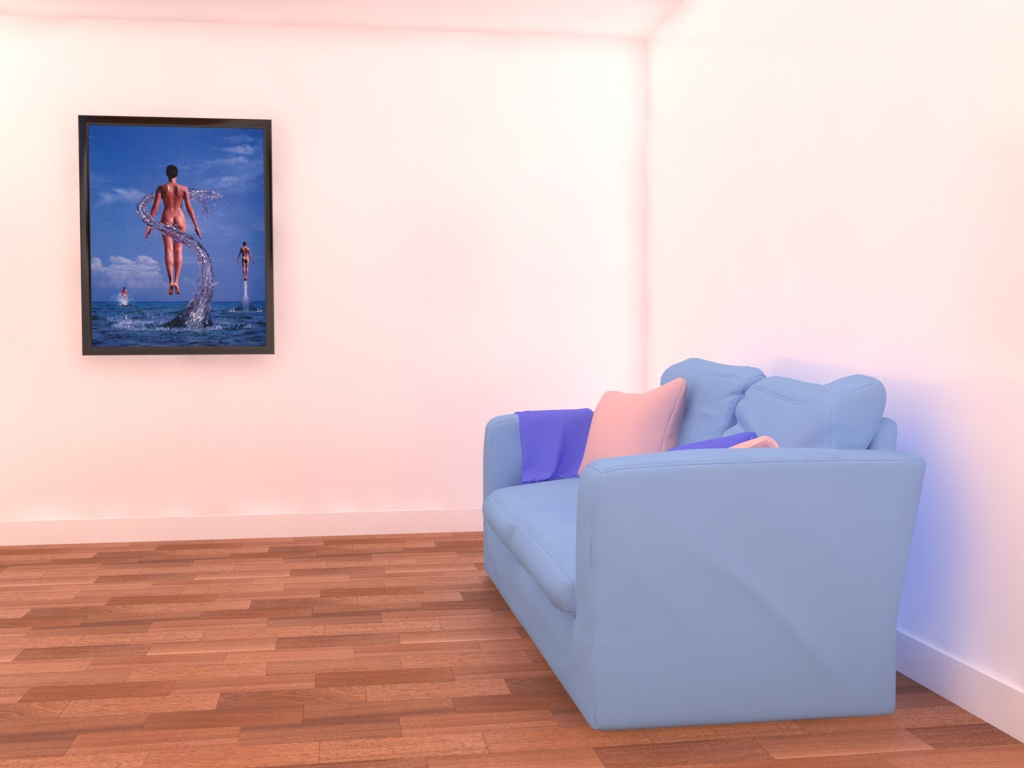
\includegraphics[width=12cm]{inspire/ShineOnRender.jpg}
	\caption{Pink Floyd, Shine On Boxset Cover, 1992.  Note AO has been overcooked a bit on this.}
	\label{fig:ShineOnRender}
\end{figure}

The example provided is the minimum standard require to receive a passing grade.  There are a number of issues with this render.  Ambient Occlusion is too strong; colors are reflecting too strongly, and the scene is not very interesting.


\vspace{1cm}

\textbf{Images by the Masters}

\begin{figure}[h]
	\centering
		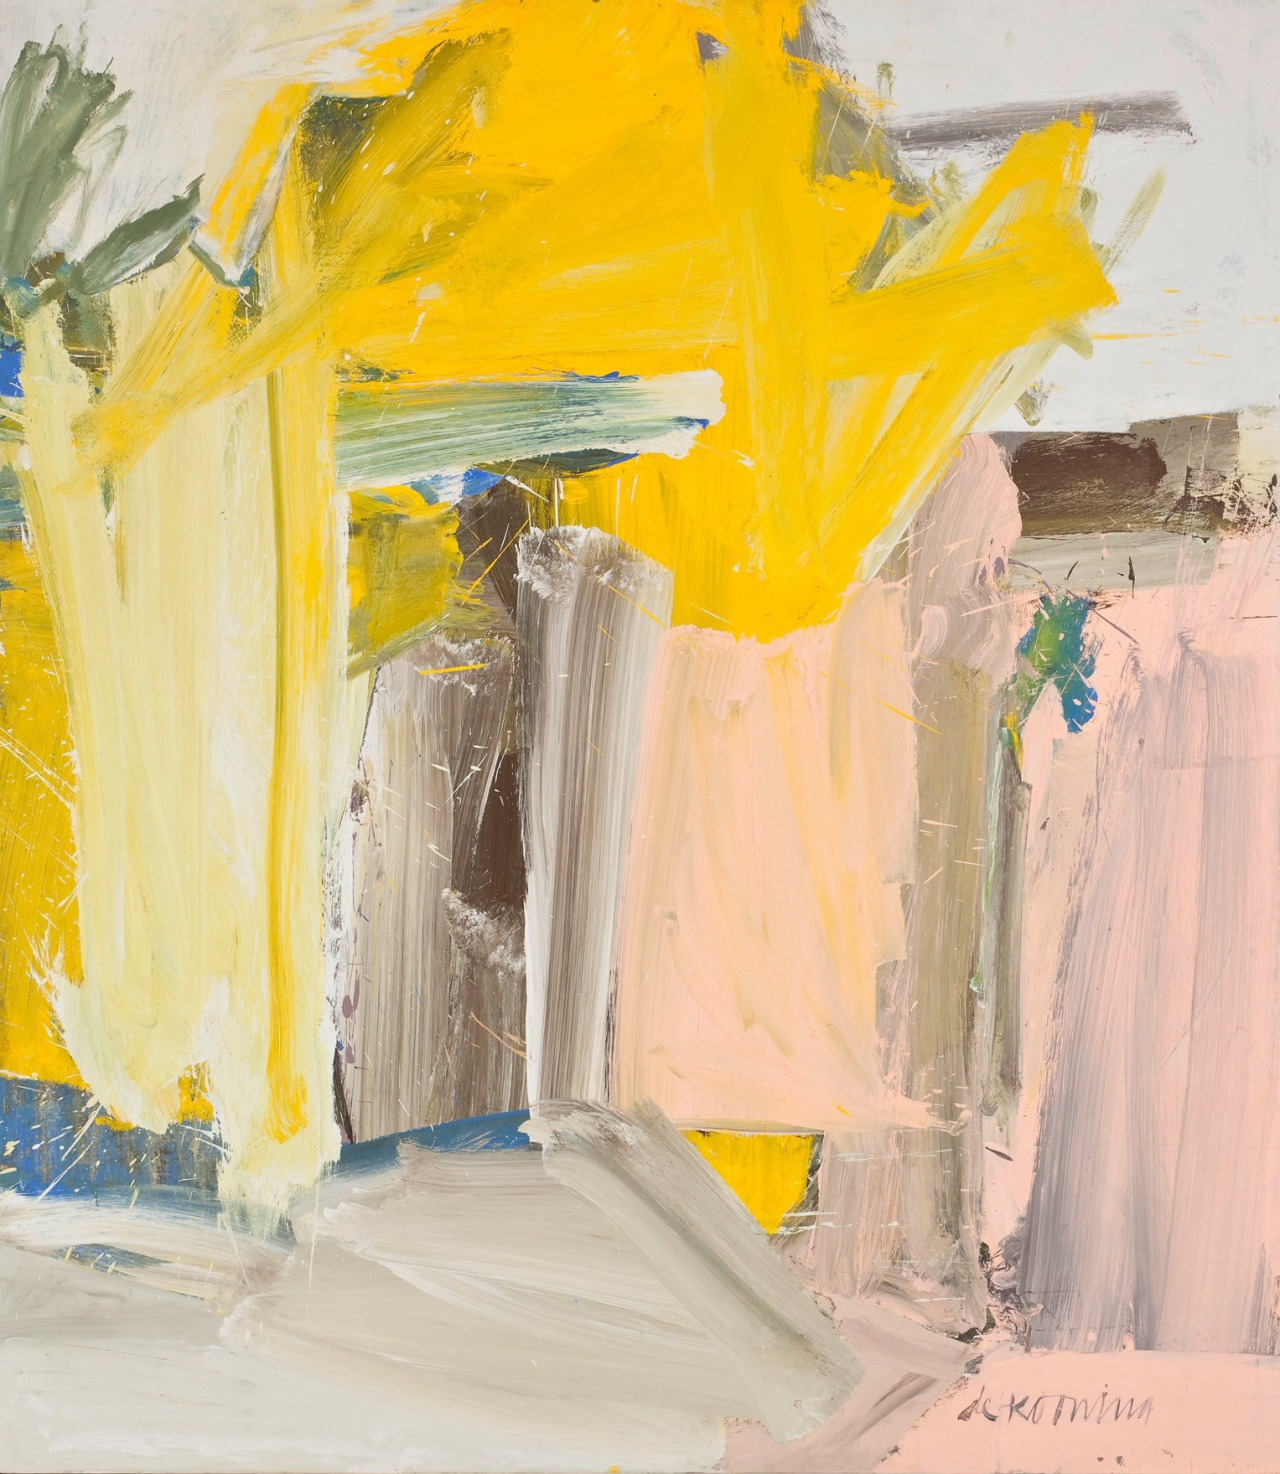
\includegraphics[width=12cm]{inspire/DoorToARiver.jpg}
		\caption{Door to a River, Willem de Kooning, 1960}
	\label{fig:DoorToARiver}
\end{figure}


\begin{figure}[h]
	\centering
	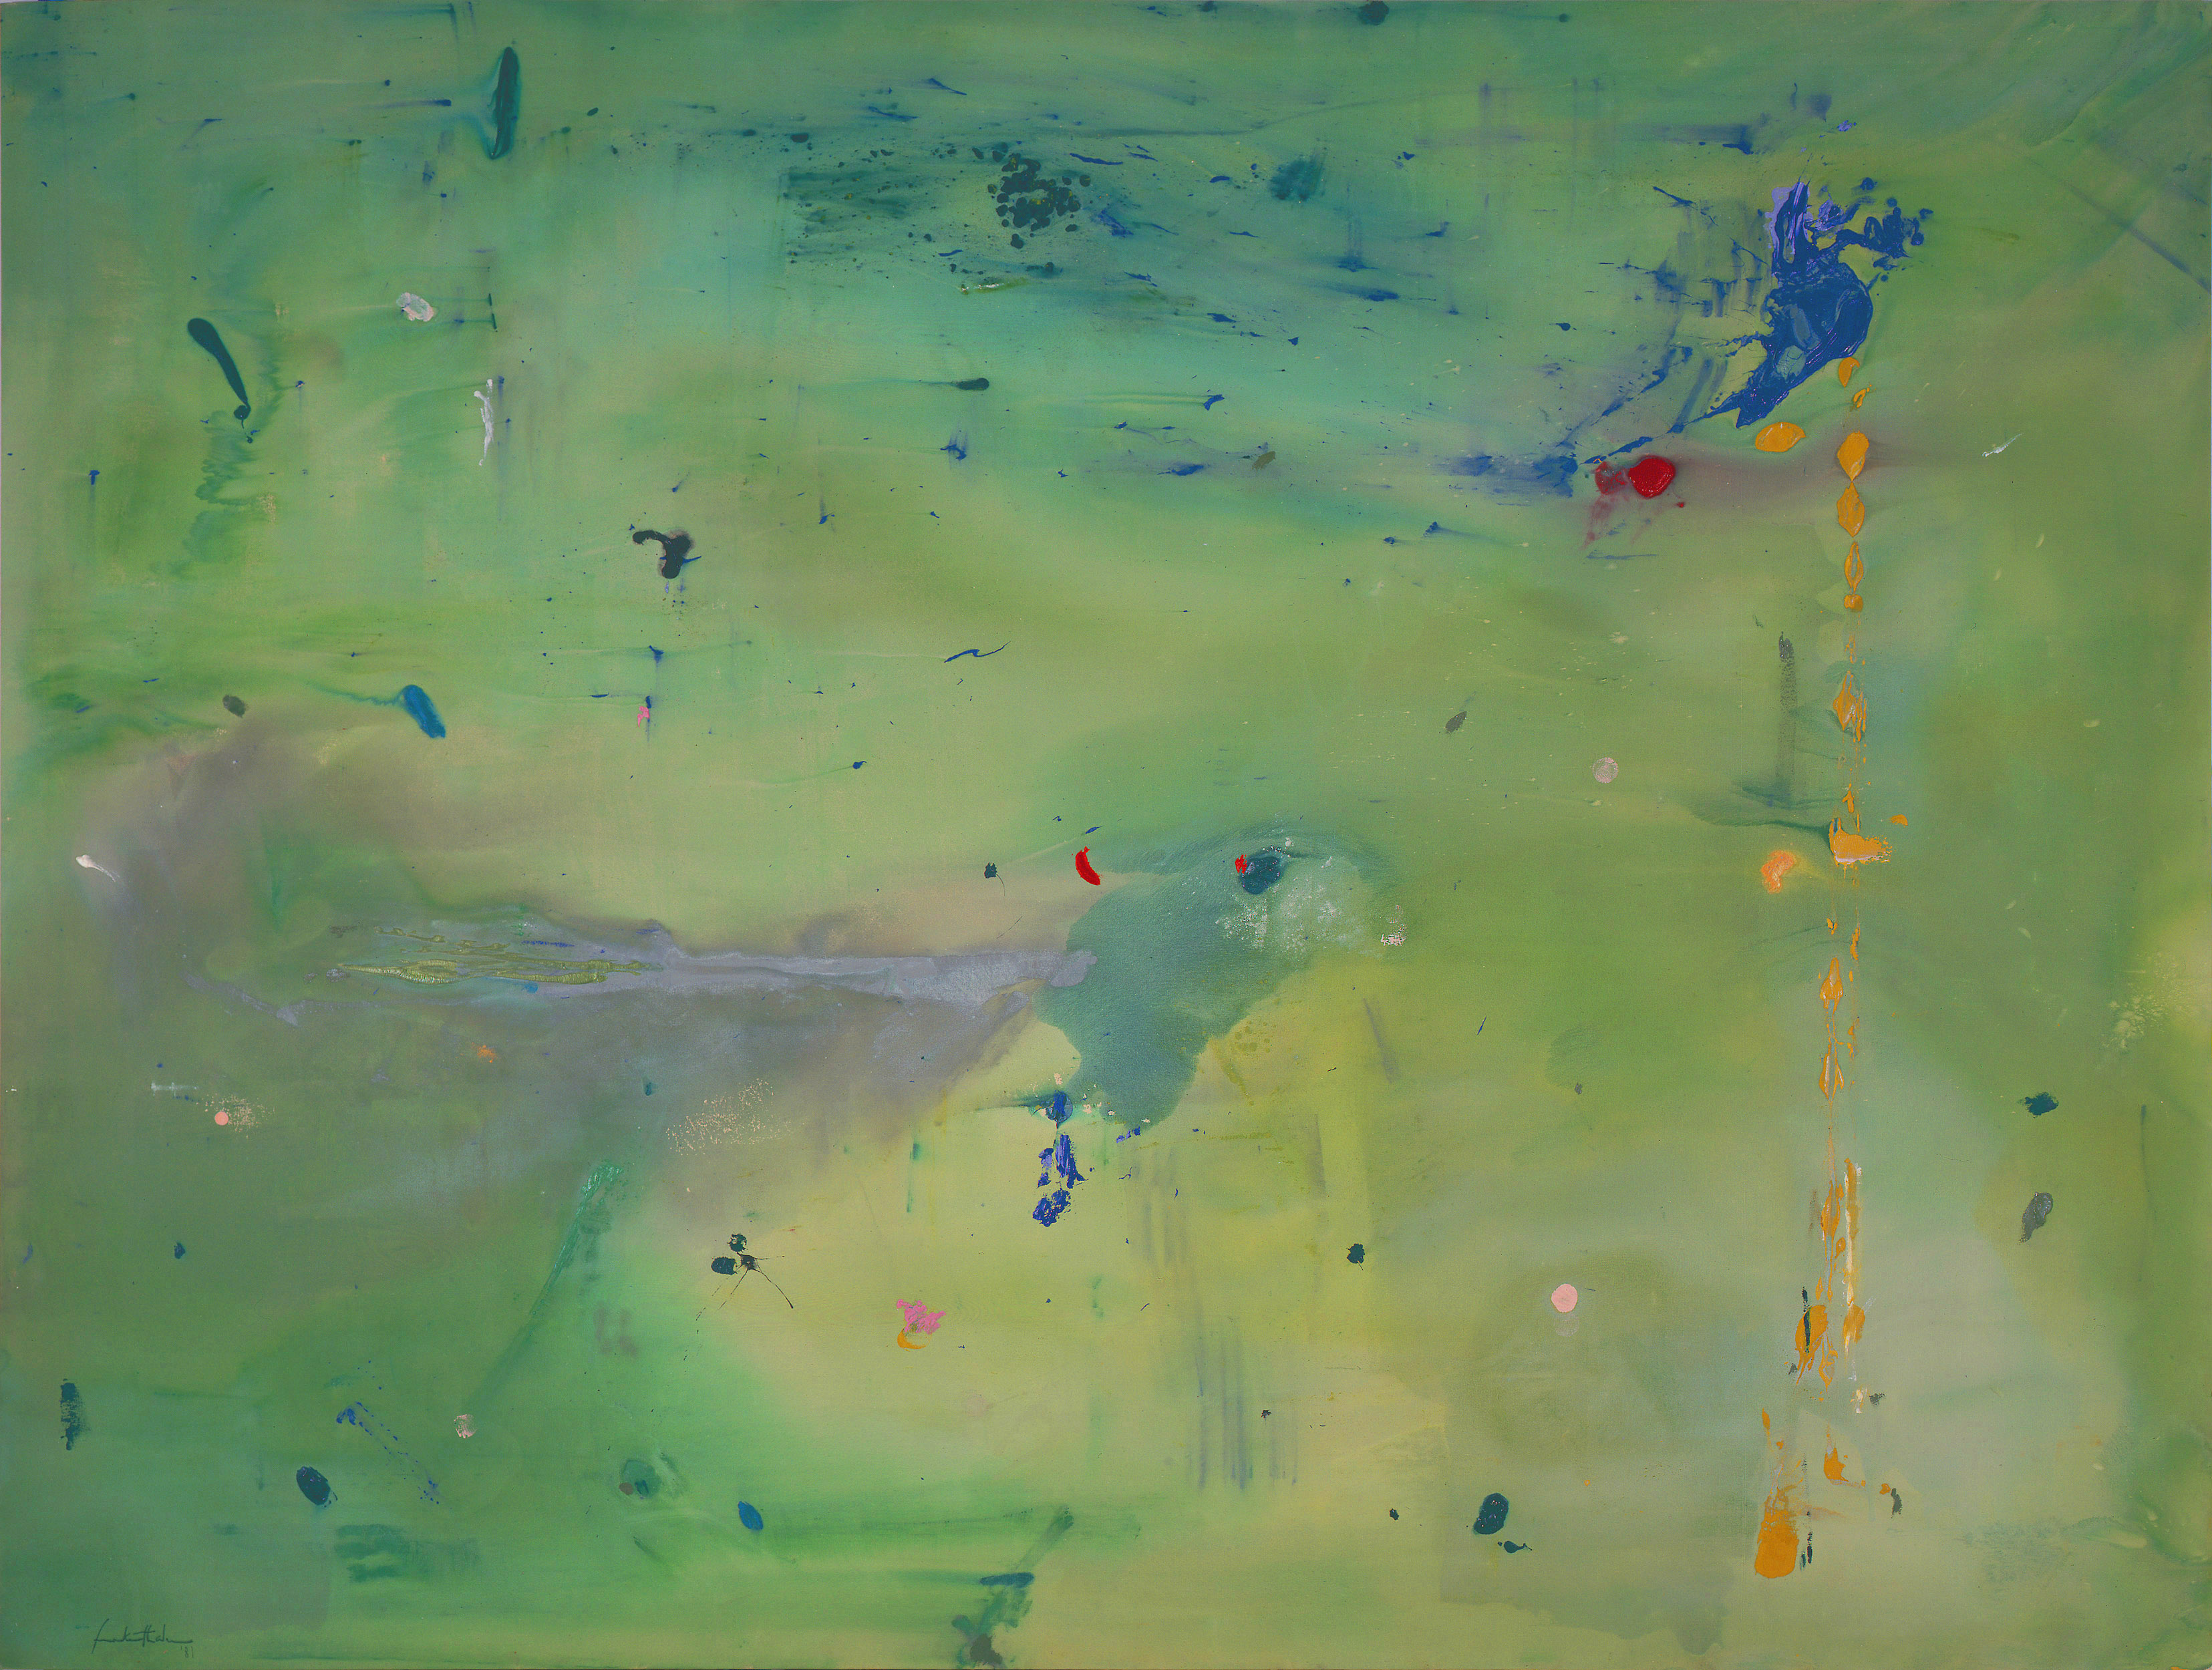
\includegraphics[width=12cm]{inspire/frankenthaler_ca27958.jpg}
	\caption{Helen Frankenthaler, A green thought in a green shade, 1981}
	\label{fig:GreenThought}
\end{figure}




\begin{figure}[h]
	\centering
	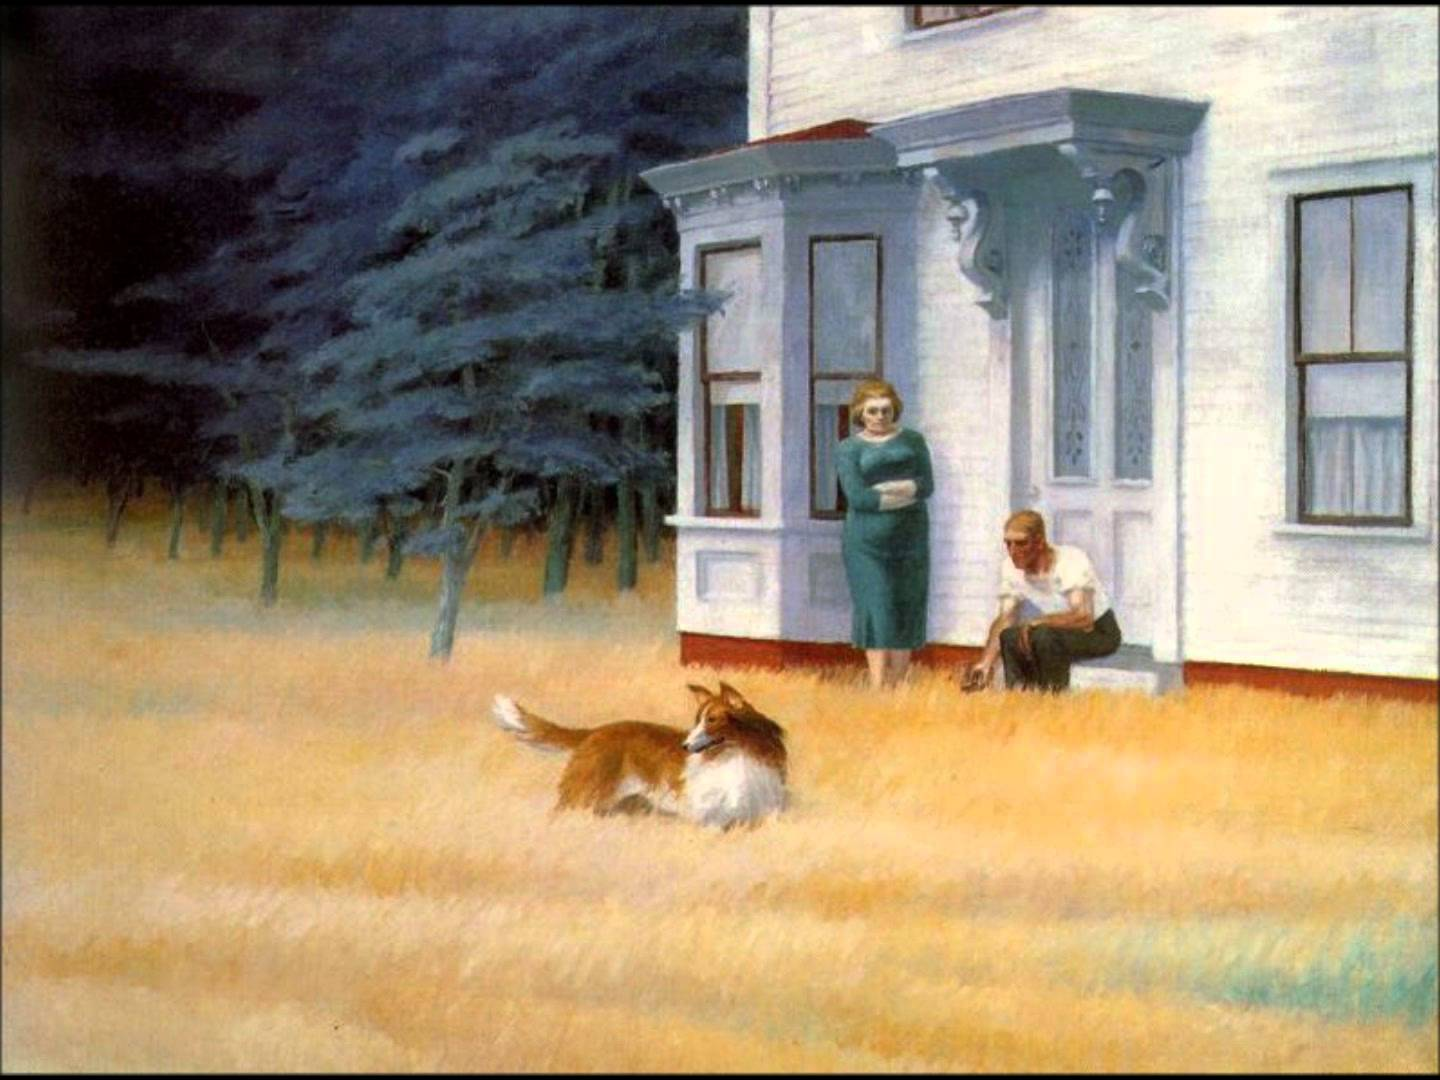
\includegraphics[width=12cm]{inspire/CapeCod.jpg}
	\caption{Edward Hopper, Cape Cod Evening, 1939}
	\label{fig:CapeCod}
\end{figure}




\begin{figure}[h]
	\centering
	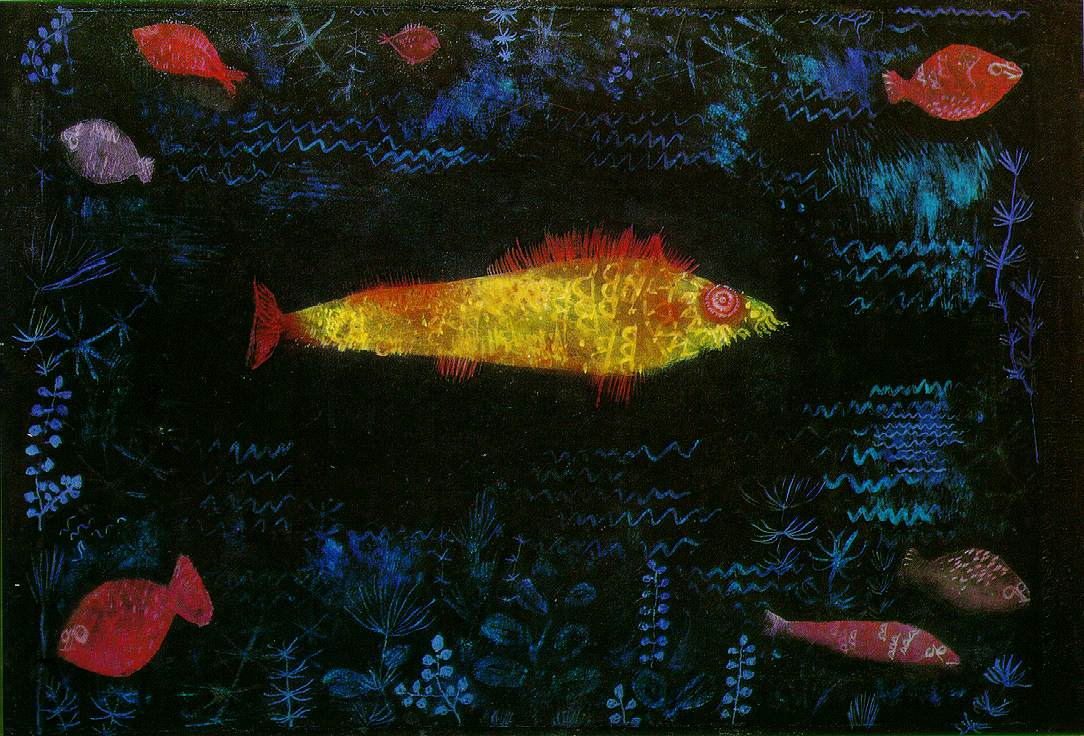
\includegraphics[width=12cm]{inspire/the-goldfish-1925.jpg}
	\caption{Paul Klee, The Golden Fish 1925}
	\label{fig:GoldenFish}
\end{figure}


\begin{figure}[h]
	\centering
	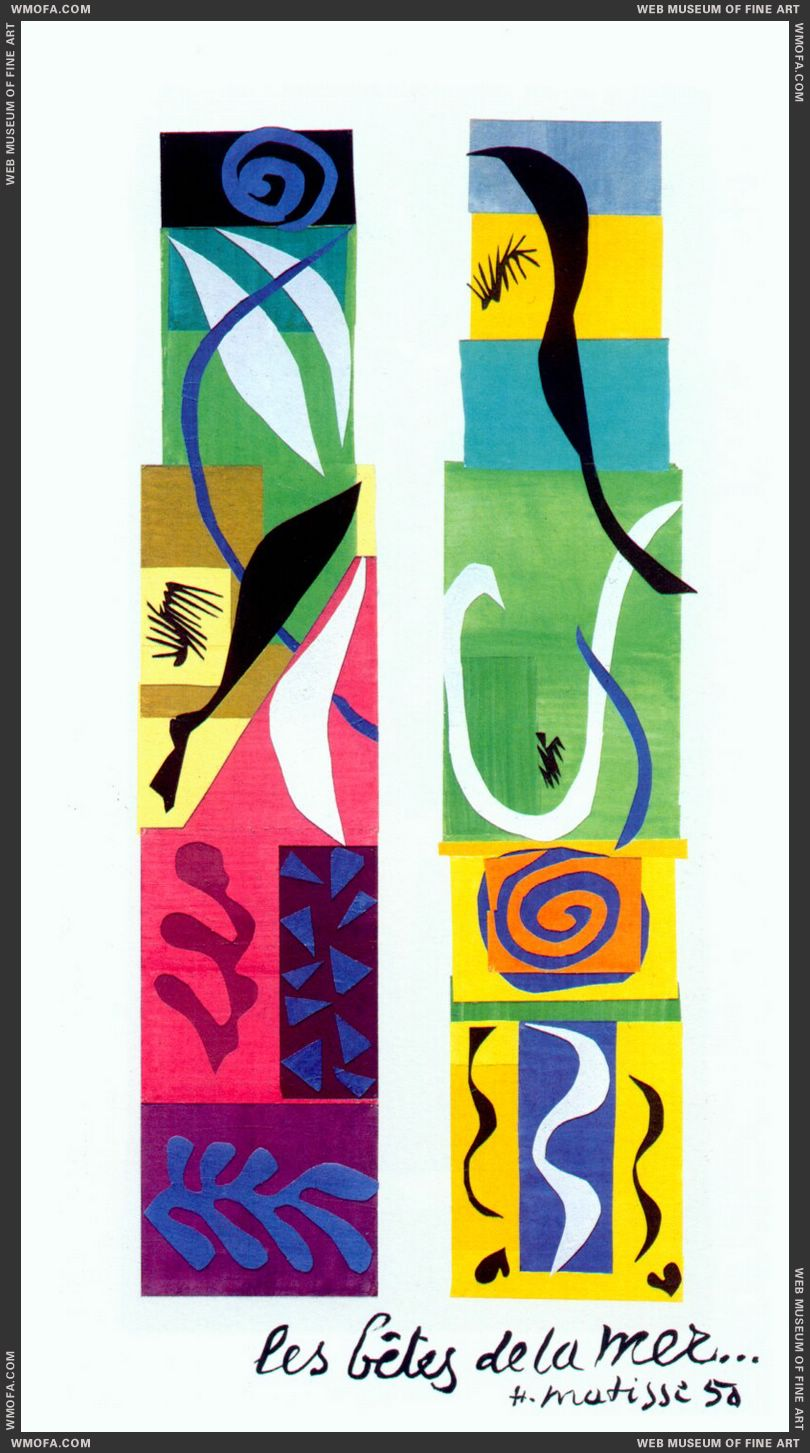
\includegraphics[width=12cm]{inspire/BeastSea.jpg}
	\caption{Henri Matisse, Beasts of the Sea, 1950}
	\label{fig:MatisseBeastsofSea}
\end{figure}


\begin{figure}[h]
	\centering
	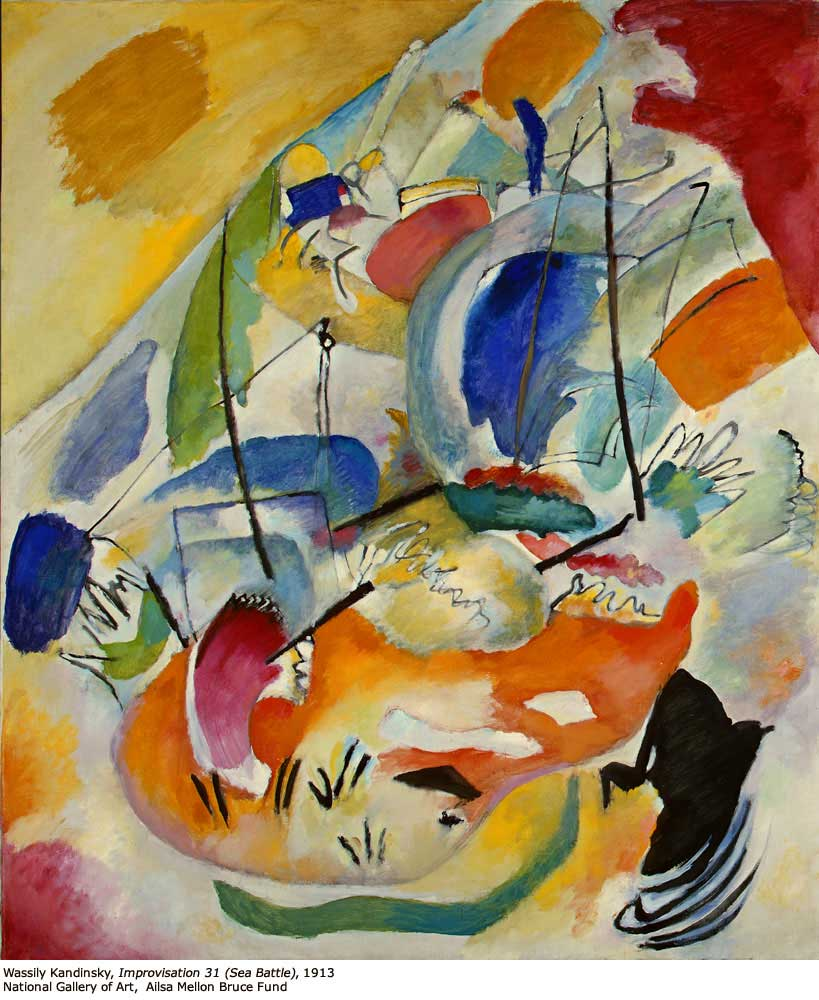
\includegraphics[width=12cm]{inspire/Improv31.jpg}
	\caption{Wassily Kandinsky, Improvisation 31, 1913}
	\label{fig:KandinskyImprov31}
\end{figure}



\begin{figure}[h]
	\centering
	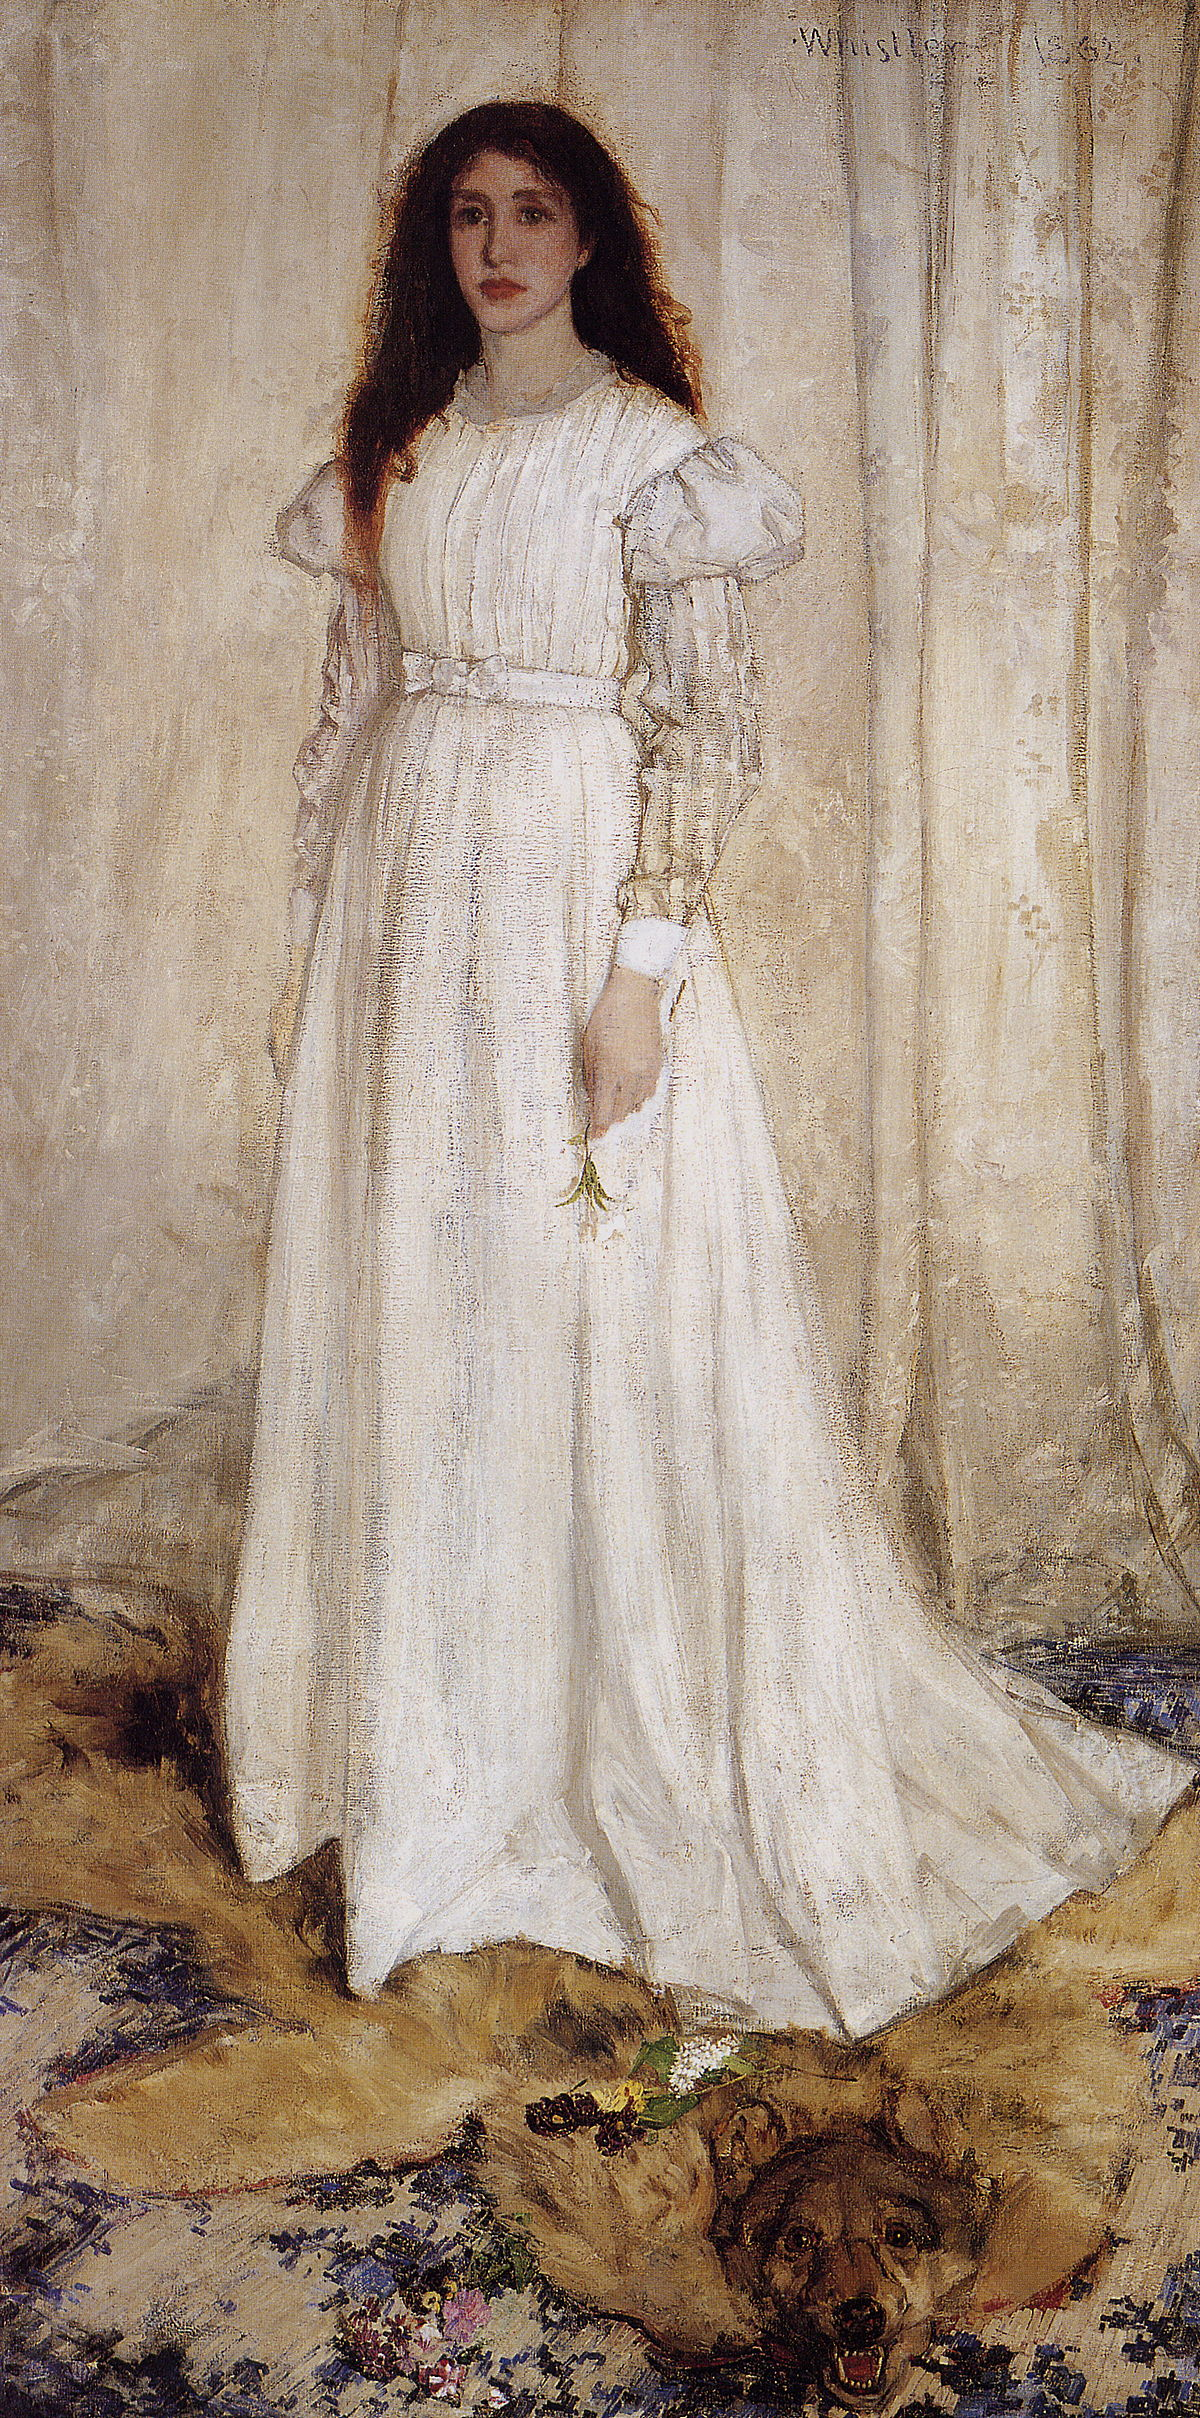
\includegraphics[width=12cm]{inspire/WhiteGirl.jpg}
	\caption{James Whistler, The White Girl, 1862}
	\label{fig:WhireGirl}
\end{figure}


\begin{figure}[h]
	\centering
	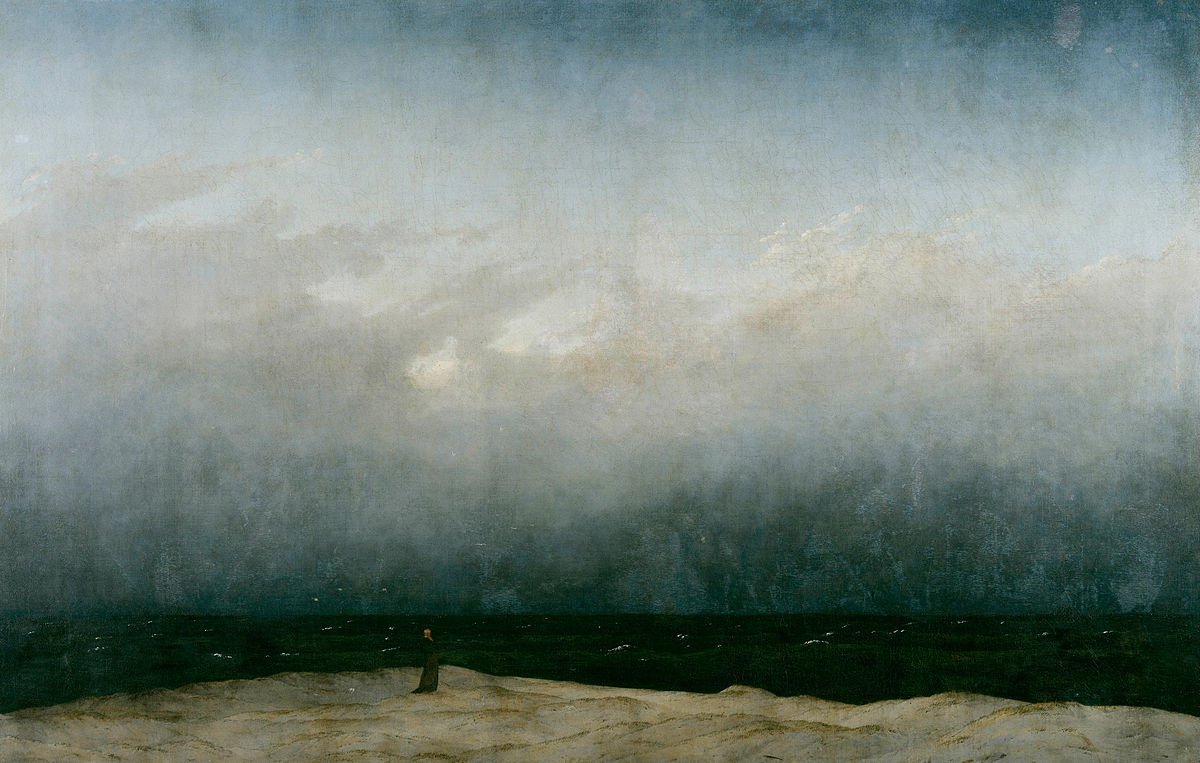
\includegraphics[width=12cm]{inspire/MonkShore.jpg}
	\caption{Caspar David Friedrich, Monk by the Shore, 1810}
	\label{fig:MonkByShore}
\end{figure}


\begin{figure}[hb]
	\centering
	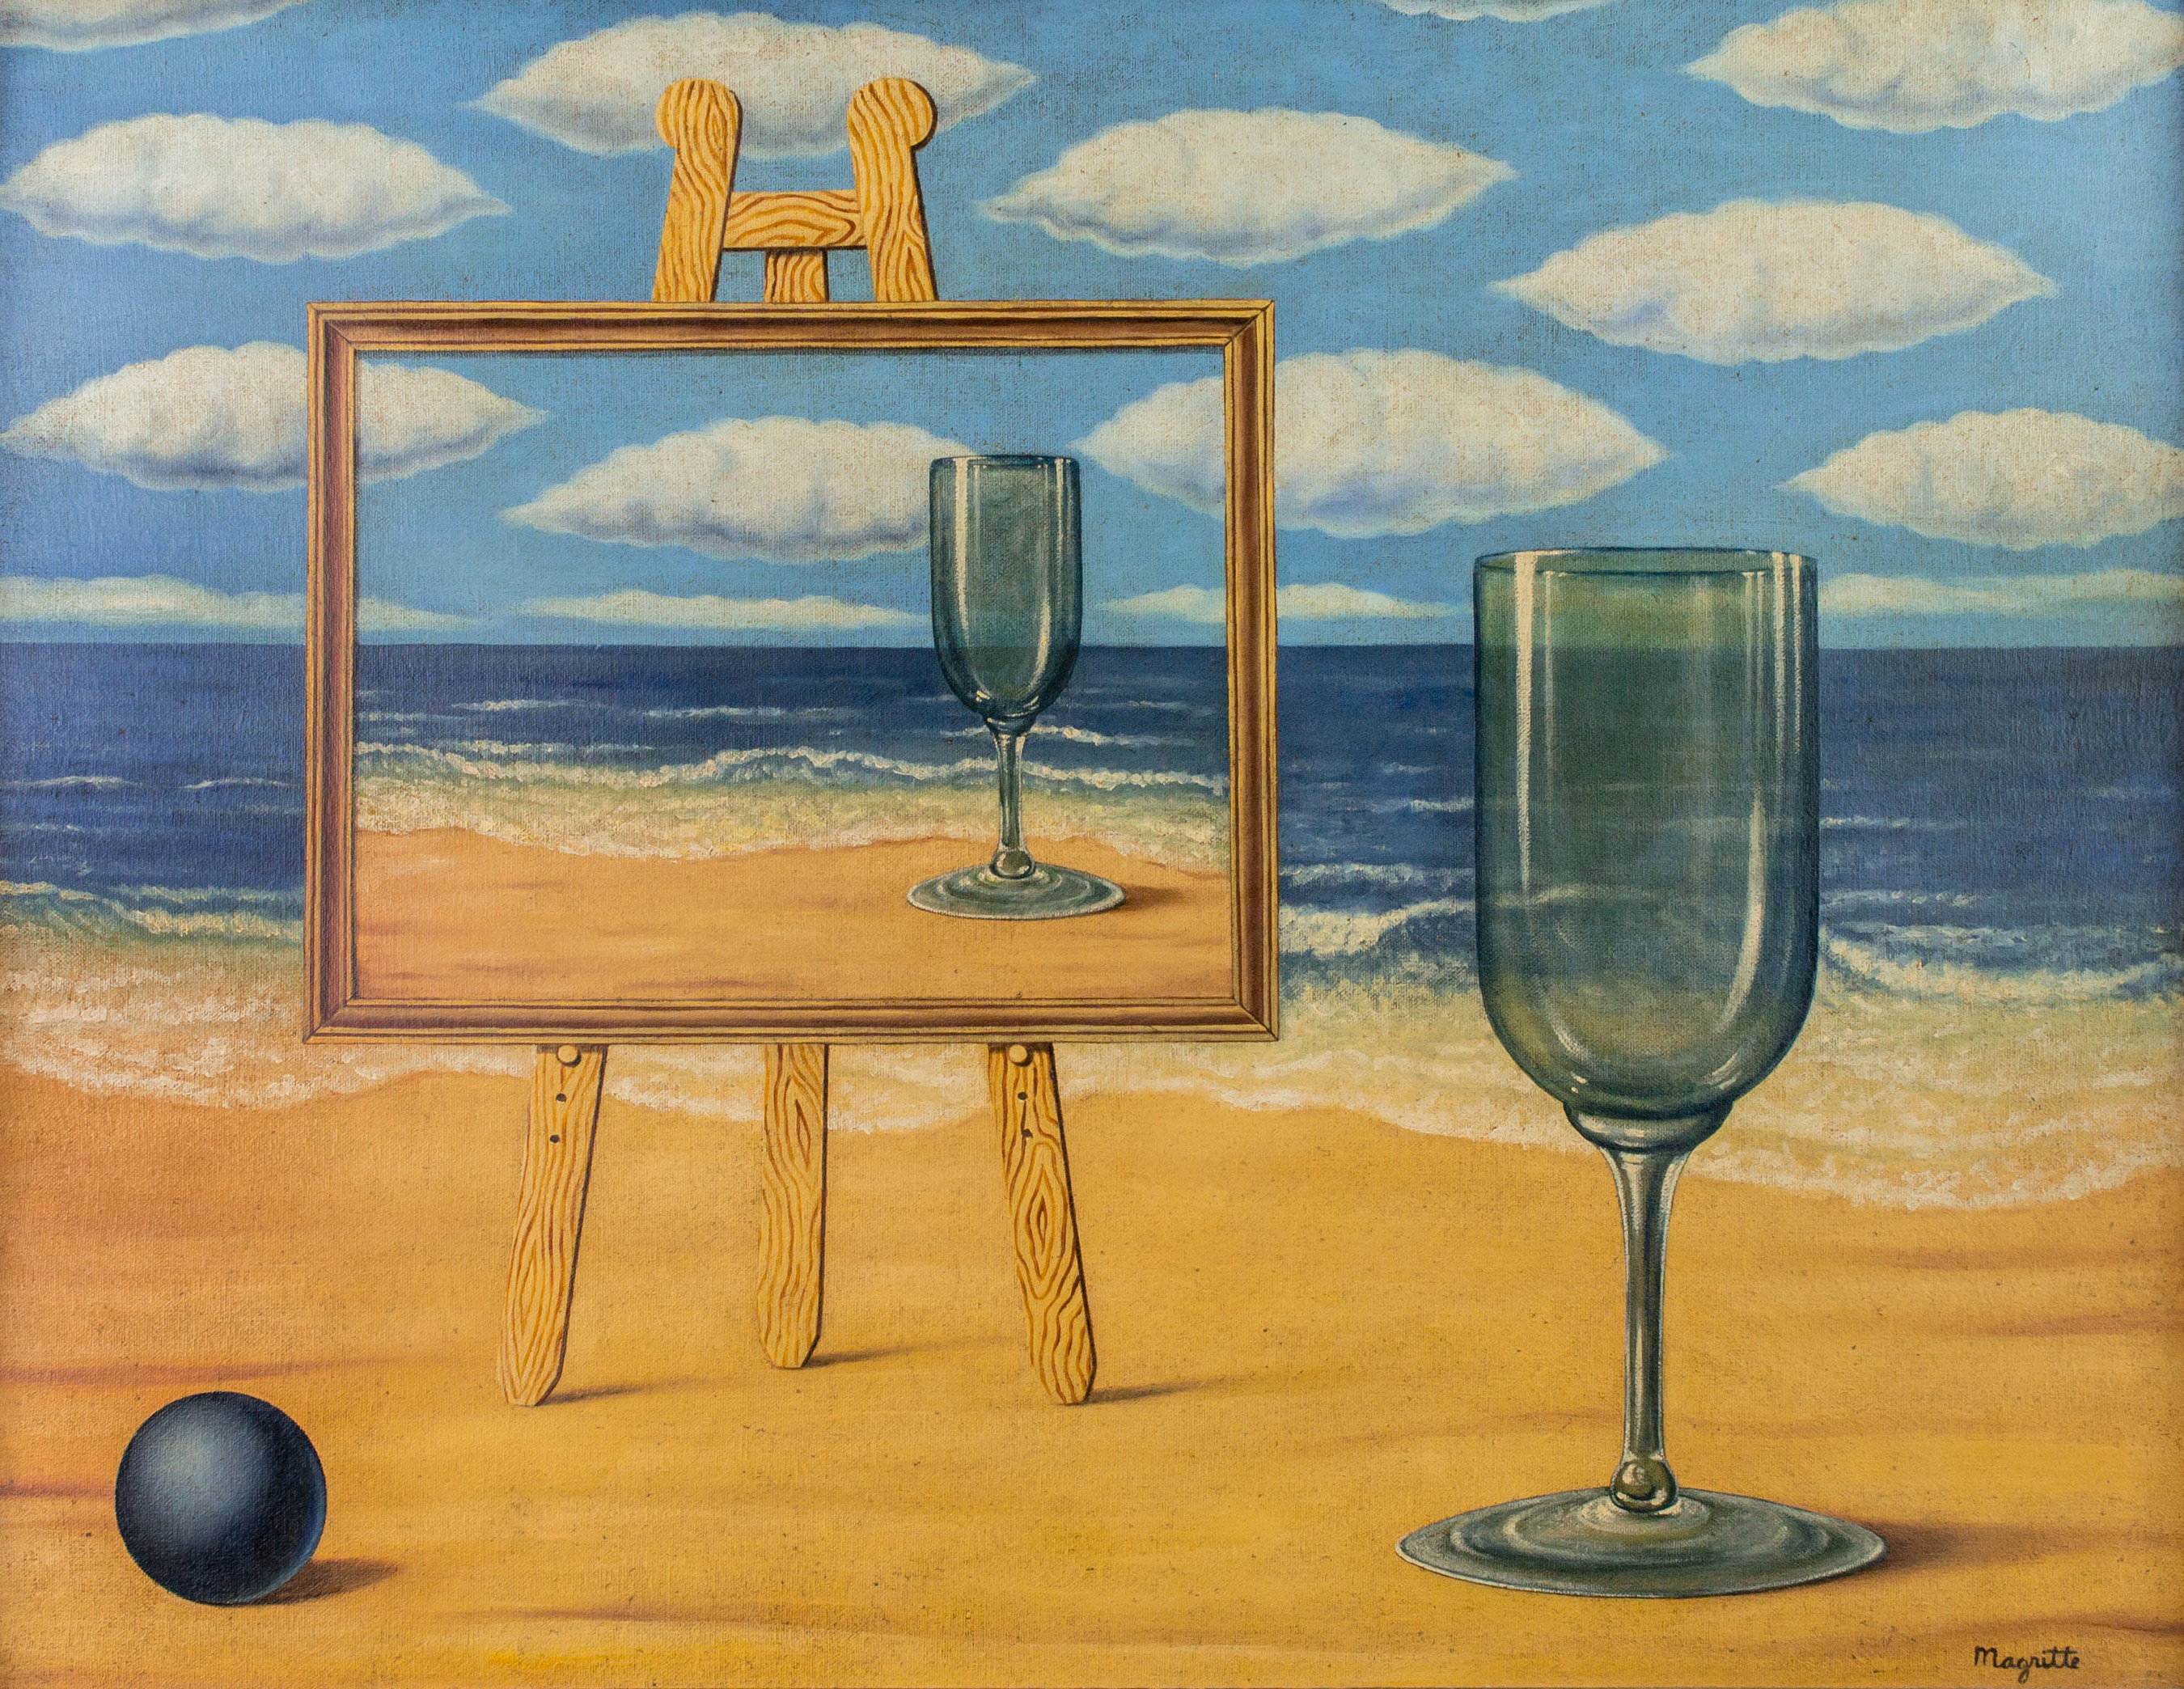
\includegraphics[width=12cm]{inspire/Magritte.jpg}
	\caption{Rene Magritte, Unknown, Unknown}
	\label{fig:Magritte}
\end{figure}


\begin{figure}[hb]
	\centering
	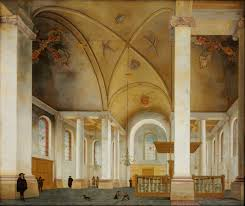
\includegraphics[width=12cm]{inspire/PieterSaenredam.jpg}
	\caption{Pieter Saenredam, Interior of the Nieuwe or St. Annakerk in Haarlem, 1653}
	\label{fig:PieterSaenredam}
\end{figure}


\vspace{1cm}
\textbf{How to Structure your Submission}
\\
All submission are to take the form of a single zip file.  The zip file must maintain the folder structure as generated by 3DS Max or Unity.   The images below, figure \ref{fig:3dsstructure} and figure \ref{fig:unity} give an indication of the folder structure that you should zip and submit.\\ \\

\begin{figure}[h]
	\centering
	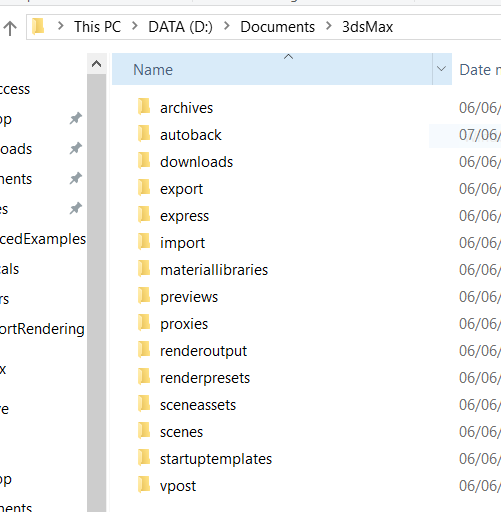
\includegraphics[width=0.5\linewidth]{img/3dsStructure.jpg}
	\caption{3D Studio Max Project Folder Structure}
	\label{fig:3dsstructure}
\end{figure}
\begin{figure}[h]
	\centering
	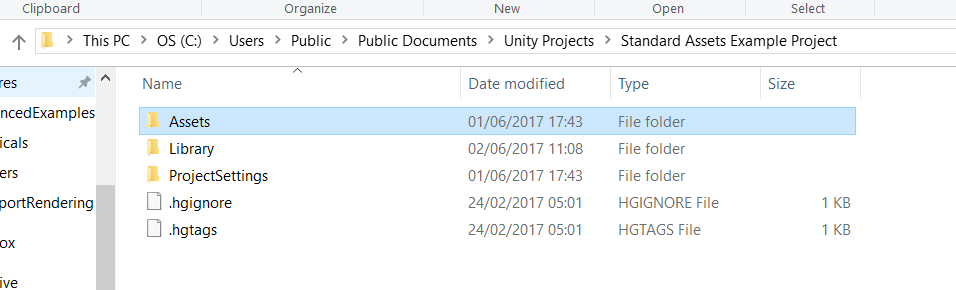
\includegraphics[width=0.9\linewidth]{img/Unity.jpg}
	\caption{Unity Game Engine File Structure}
	\label{fig:unity}
\end{figure}

All assets used during the course of the assignment are to be submitted.  All assets used and created should be placed within the appropriate folder.  To clarify, all 3ds Scene files should be placed within the 'scenes' folder; and all renders should be placed within the 'renderoutput' folder.
\\
\\
Please note that it is not appropriate to submit a single \textit{.max} file, single \textit{.jpg} file, or a single \textit{.unity} file.  

\vspace{1cm}
\textbf{Late Submission}\\
Failure to submit your assignment on or before the date and time indicated on Moodle will result in a penalty of 5\% per day or part thereof.
\\
\\
Late submission penalties will not apply in cases where a valid medical certificate is provided.  In such instances an extension of time will be granted for the duration of illness stated on the medical certificate that falls after the submission date.  A copy of the medical certificate must be included with the late submission.
\\
\\
Late submission penalties may also be avoided in exceptional circumstances.  These will be dealt with on a case by case basis.  Please note that loss of pen-drives, inability to use or access the software etc. will not be considered 'exceptional circumstances'.




\end{document}